\documentclass{scrartcl}
	\usepackage[latin1]{inputenc}
	\usepackage{fourier}
	\usepackage{graphicx}
	\usepackage{xcolor}
	\usepackage{tikz}
	\usepackage{ifthen}
	\usepackage{paralist}
	\usepackage{animate}
	\usepackage{lipsum}
	\usepackage{amsmath}
	\usepackage{listings}
	%\usepackage[square]{natbib}
		
	\usetikzlibrary{calc}
	
	\newcommand{\scalefactor}{10}
	\tikzset{box/.style={color=#1,thick},box/.default=red}
	\tikzset{letter/.style={color=#1,inner sep=0pt},letter/.default=gray!50}
	\tikzset{baseline/.style={color=#1,thin},baseline/.default=blue}
	
% Configura��es personalizadas do c�digo LaTeX.	
\lstnewenvironment{LaTeXcode}{
	\setlength{\abovecaptionskip}{0pt}
	\lstset{language=[LaTeX]TeX}
	\lstset{%
		basicstyle=\footnotesize\ttfamily,  % Global
		keywordstyle=\color{blue}\bfseries, % Comandos
		identifierstyle=,                   % Texto
		stringstyle=,                       % Strings 
		commentstyle=\color{gray},          % Coment�rios
		showstringspaces=false,             % Espa�os
		rulecolor=\color{gray},             % Linha da caixa
	}
}% Abrindo o ambiente.
{}% Fechando o ambiente.	
	
	\newcommand\fileext[1]{{\ttfamily #1}}
	
	\newboolean{animate}
	\setboolean{animate}{true}
	
	\title{\makebox[0pt][l]{\scalebox{1}[-1]{\raisebox{\depth}{\color{blue!25}Boxes and more boxes}}}%
		\raisebox{\depth}{Boxes and more boxes}}
	\author{I. R. Pagnossin}
	
	\newcommand{\cs}[2][\null]{%
		\ifthenelse{\equal{#1}{\null}}%
		{\textsf{\textbackslash #2}}%
		{\textsf{\textbackslash #2\{#1\}}}%
	}
	
	\newcommand{\pkg}[1]{\textsf{#1}}
	\newcommand{\foreign}[1]{\textsl{#1}}
	\newcommand{\env}[1]{\textsf{#1}}
	\newcommand{\boxct}[1]{\textbf{#1}}
	
	\newcommand{\B}[1]{{\color{red!30}\fbox{\textcolor{black}{#1}}}}
	
	\setlength\fboxsep{0pt}
	
	\hyphenation{e-qua-tion rec-tan-gles un-break-a-ble de-fined im-me-di-ate-ly}
\begin{document}
	

	\maketitle

	\begin{abstract}
		Boxes are a key concept in \TeX/\LaTeX\ as well as an useful tool, though not a very well known one. I believe this is due to the success of \LaTeX\ in providing a high level interface to \TeX, which allows the user to produce beautiful documents without getting acquainted with the concept of boxes. But it is useful to know the box concept because it enhances our understanding of \TeX, helps us to avoid and solve problems and even can propose solutions for unusual circumstances.
		
		In this paper we reproduce, step by step, the reflection effect in the title of this job in order to gain some knowledge of the box concept.
	\end{abstract}
	
	Among the fundamental ingredients of a \LaTeX\ document, there are \emph{boxes:} imaginary rectangles which enclose letters, lines, pages, paragraphs, figures, tables etc. Indeed, \TeX\ does not typeset letters or characters, lines\dots\ but boxes!
	
	You probably already used boxes to avoid breaking some word or maybe to frame an equation. But they are far more useful than this. A simple but instructive example is the reflection effect in the title of this paper, which requires one customized box. Let's learn something from it.
	
	Figure~\ref{fig:g} shows the box associated with the letter \boxct{g}. It has three dimensions: \emph{height}, \emph{width} and \emph{depth}. It is these dimensions that \LaTeX\ actually cares about, not the content of the box. In other words, \LaTeX\ does not ``see'' the letter \boxct{g}, only its box. This is the important fact to understand.
	
	\begin{figure}
		\centering
		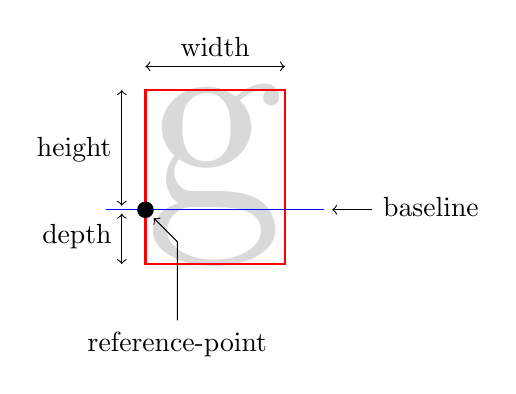
\begin{tikzpicture}

	% A letra "g" e sua caixa
	\node [letter] (g) at (2,0) {\scalebox{\scalefactor}
		{\color{gray!30}g}};
	\draw [box] (g.south west) rectangle (g.north east);
	
	\coordinate (base line left)  at ($(g.base west) - (5mm,0)$);
	\coordinate (base line right) at ($(g.base east) + (5mm,0)$);
	
	% A linha-base
	\draw [baseline] (base line left) -- (base line right);
			
	% A flecha e o r�tulo "Linha-base"
	\draw [<-] ($(base line right) + (1mm,0)$) -- ++(5mm,0)
		node [inner sep=0mm, label=right:\raisebox{0.5ex}{baseline}] {};
	
	% O ponto-de-refer�ncia
	\fill [black] (g.base west) circle (3pt);
	
	% Flecha da altura
	\draw [<->] ($ (g.base west) + (-3mm,+0.5mm) $) --
	            ($ (g.north west) + (-3mm,0) $);
	
	% Flecha da profundidade
	\draw [<->] ($ (g.south west) + (-3mm,0) $) -- 
	            ($ (g.base west) + (-3mm,-0.5mm) $);

	% Flecha da largura
	\draw [<->] ($ (g.north west) + (0,3mm) $) --
	            ($ (g.north east) + (0,3mm) $);
	            
	% Flecha da altura total
%	\draw [<->] ($ (g.south east) + (3mm,0) $) --
%	            ($ (g.north east) + (3mm,0) $);
	
	% R�tulo "Altura"
	\node [inner sep=3mm, label=left:height]
		at ($ (g.base west)  ! 0.5 ! (g.north west) $) {};
	
	% R�tulo "Profundidade"
	\node [inner sep=3mm, label=left:depth]
		at ($ (g.base west)  ! 0.5 ! (g.south west) $) {};
	
	% R�tulo "Largura"
	\node [inner sep=3mm, label=above:width]
		at ($ (g.north west) ! 0.5 ! (g.north east) $) {};
	
	% Flecha e r�tulo "Ponto-de-refer�ncia"
	\draw [<-] ($(g.base west) + (3pt,-3pt)$) -- ++(3mm,-3mm) -- ++(0mm,-1cm)
		node [circle,inner sep=0mm,label=below:reference-point] {};
	
\end{tikzpicture}
		\caption{the dimensions of a box. Everything that is visible in a document produced by \LaTeX\ is in one or more boxes, which is why they are so fundamental.}	
		\label{fig:g}
	\end{figure}
	
	We can ask \LaTeX\ to show us this box: just write \cs[g]{framebox} (first you must set \cs{fboxsep} to zero, in order to remove the extra space around \boxct{g}: \verb|\setlength{\fboxsep}{0in}|).
	
	Much more important than just showing the box, \cs{framebox} builds a box with whatever you want inside it. For instance, \cs[Boxes]{framebox}. Now \boxct{Boxes} is a \emph{single} box, as unbreakable as the letter \boxct{g} itself. By the way, this is another property to keep in mind: \emph{boxes cannot be broken}.
	
	Another interesting property is this: \emph{the contents of a box need not lie inside it}. You may have noticed that, given the content as an argument, the command \cs{framebox} adjusts the dimensions of the box to that of the contents (in reality, to the ``sub-boxes'' that compose the contents). But you can define them as well. For example,
	
	\begin{center}
		\verb|\framebox[1in]{Boxes}|
	\end{center}

	\noindent produces \framebox[1in]{Boxes}, a box one inch wide. That is, a box which occupies more space than its contents. You can also define the alignment of the content with the box, to the left, center or right, as shown \ifthenelse{\boolean{animate}}{in the animation}{\unskip} below:
		
	\smallskip
	
	\ifthenelse{\boolean{animate}}
	{\noindent\begin{animateinline}[loop]{1}
			\colorbox{yellow!30}{\makebox[\textwidth]{\rule[-1ex]{0pt}{4ex}%
				\texttt{\textbackslash framebox[1in][\textcolor{red}{l}]\{Boxes\}}\qquad produces\qquad\framebox[1in][l]{Boxes}}}
			\newframe
			\colorbox{yellow!30}{\makebox[\textwidth]{\rule[-1ex]{0pt}{4ex}%
				\texttt{\textbackslash framebox[1in][\textcolor{red}{c}]\{Boxes\}}\qquad produces\qquad\framebox[1in][c]{Boxes}}}
			\newframe
			\colorbox{yellow!30}{\makebox[\textwidth]{\rule[-1ex]{0pt}{4ex}%
				\texttt{\textbackslash framebox[1in][\textcolor{red}{r}]\{Boxes\}}\qquad produces\qquad\framebox[1in][r]{Boxes}}}					
		\end{animateinline}}
	{\begin{compactitem}
		\item {\ttfamily\textbackslash framebox[1in][\textcolor{red}{l}]\{Boxes\}} produces \framebox[1in][l]{Boxes}
		\item {\ttfamily\textbackslash framebox[1in][\textcolor{red}{c}]\{Boxes\}} produces \framebox[1in][c]{Boxes}
		\item {\ttfamily\textbackslash framebox[1in][\textcolor{red}{r}]\{Boxes\}} produces \framebox[1in][r]{Boxes}
	\end{compactitem}}
		
	\smallskip
	
	In a similar fashion, we may create a box which occupies less space than its contents; a zero-width box, for instance:
	
	\begin{center}
		\verb|\framebox[0in][l]{Boxes}|
	\end{center}
	
	Try it yourself and notice that \boxct{Boxes} overlaps the text to the right. This happens because, as we have seen, \LaTeX\ uses the dimensions of the letters (boxes) to place them side by side in a row. However, the box we have just created occupies no (horizontal) space\dots\ it looks like it is not there, though its contents are (try also changing the alignment parameter).

	Another command we need to produce the reflection effect is the \cs{scalebox}, defined in the package \pkg{graphicx}. Its syntax is \verb|\scalebox{|$f_x$\verb|}[|$f_y$\verb|]{|\emph{a box}\verb|}|. It changes the dimensions of the box \emph{and its contents} according to the horizontal and vertical scaling factors $f_x$ and $f_y$ (respectively) and creates a new box that encloses this new content. In our case, in order to get {\bfseries\scalebox{1}[-1]{Boxes}Boxes} we write
	
	\begin{center}
		\verb|\scalebox{1}[-1]{Boxes}Boxes|
		\marginpar{\scalebox{1}[-1]{Boxes}Boxes}
	\end{center}

	This means we instruct \LaTeX\ to multiply the width by $f_x = 1$ (hence, nothing changes on horizontal) and the height ($> 0$) and the depth ($= 0$) by $f_y = -1$. As a result, we have a vertical reflection of \boxct{Boxes}. A hint: the commands defined by \pkg{graphicx} receive boxes as arguments, not just figures (which are boxes too). Since the package itself was designed to handle figures, it is quite common to think that its commands apply only to figures, but this is not true.

	Lets proceed. How can we place \textbf{\scalebox{1}[-1]{Boxes}} below \boxct{Boxes}? Simple: just contstruct it in a way that occupies no horizontal space, that is, just put it in a zero-width box:
	
	\begin{center}
		{\ttfamily
		\textbackslash makebox[0in][l]\{%
			{\color{gray}\textbackslash scalebox\{1\}[-1]\{Boxes\}\textcolor{black}{\}}%
				Boxes}%
		}
		\marginpar{\makebox[0in][l]{\scalebox{1}[-1]{Boxes}}Boxes}
	\end{center}
	
	Here we swapped \cs{framebox} by \cs{makebox}. These two commands are equivalent, except that the former draws a frame around the box, while the latter does not.
	
	Finally, we choose the reflection color (use the package \pkg{xcolor}):
	
	\begin{center}
		{\color{gray}\ttfamily \cs{makebox}[0in][l]\{\cs{scalebox}\}\{1\}[-1]\{\color{black}\cs[blue!30]{textcolor}\{\textcolor{gray}{Boxes}\}\color{gray}\}Boxes}
		\marginpar{\makebox[0in][l]{\scalebox{1}[-1]{\textcolor{blue!30}{Boxes}}}Boxes}
	\end{center}
	
	The \ifthenelse{\boolean{animate}}{animation}{sequence} below illustrates the changing of the box width, from its \emph{natural width} (defined by the content) down to zero. Notice that the non-inverted \boxct{Boxes} always starts immediately after the frame (the box), not after the content (\raisebox{\depth}{\scalebox{1}[-1]{\textcolor{blue!30}{Boxes}}}).
			
	\ifthenelse{\boolean{animate}}
	%-- Anima��o HABILITADA.
	{\smallskip
			{\Huge
			\noindent\begin{animateinline}[loop]{10}
			\multiframe{20}{Rf=1+-0.05}{%
				\colorbox{yellow!30}{\makebox[\textwidth]{\rule[-2ex]{0pt}{4ex}%
				\framebox[\Rf\width][l]{\scalebox{1}[-1]{\textcolor{blue!30}{Boxes}}}Boxes}}%
			}
			\newframe
			\multiframe{10}{Rf=0+0.05}{%
				\colorbox{yellow!30}{\makebox[\textwidth]{\rule[-2ex]{0pt}{4ex}%
				\framebox[0\width][l]{\scalebox{1}[-1]{\textcolor{blue!30}{Boxes}}}Boxes}}%
			}			
			\newframe
			\multiframe{20}{Rf=0+0.05}{%
				\colorbox{yellow!30}{\makebox[\textwidth]{\rule[-2ex]{0pt}{4ex}%
				\framebox[\Rf\width][l]{\scalebox{1}[-1]{\textcolor{blue!30}{Boxes}}}Boxes}}%
			}
		\end{animateinline}}\smallskip}
	%-- Anima��o N�O HABILITADA.
	{%
		\medskip
		\noindent
		\framebox[1.00\width][l]{\scalebox{1}[-1]{\textcolor{blue!30}{Boxes}}}Boxes\hfill
		\framebox[0.80\width][l]{\scalebox{1}[-1]{\textcolor{blue!30}{Boxes}}}Boxes\hfill
		\framebox[0.60\width][l]{\scalebox{1}[-1]{\textcolor{blue!30}{Boxes}}}Boxes\hfill
		\framebox[0.40\width][l]{\scalebox{1}[-1]{\textcolor{blue!30}{Boxes}}}Boxes\hfill
		\framebox[0.20\width][l]{\scalebox{1}[-1]{\textcolor{blue!30}{Boxes}}}Boxes\hfill
		\framebox[0.00\width][l]{\scalebox{1}[-1]{\textcolor{blue!30}{Boxes}}}Boxes\par
		\medskip
	}
		
	There are boxes more complex than these. As I mentioned, everything that is visible in a document produced by \LaTeX\ is in one or more boxes. There are even invisible elements in your document that are boxes too. An example is the paragraph indentation, which is nothing more than an empty box of width \cs{parindent}. In any case, all of the concepts we have just seen remain valid.
	
	Let's see an example. The line below contains four boxes plus some filling lines (which are boxes too): the first one you already know, the second is an entire paragraph, the third is a figure and the fourth, a table (or a matrix, if you prefer). All of them have height, width and depth, are unbreakable and are placed side by side with their \emph{reference-points} aligned (fig.~\ref{fig:g}) over an imaginary line named \emph{baseline}, represented by the filling lines.
		
	\smallskip
		
	\noindent\hrulefill
	\makebox[0cm][l]{\scalebox{1}[-1]{\textcolor{blue!30}{Boxes}}}Boxes\hrulefill
	\fbox{\begin{minipage}{0.3\textwidth}
		\setlength{\parindent}{0.1\textwidth}
		\tiny\lipsum[11]
	\end{minipage}}\hrulefill
	\fbox{{\includegraphics[width=0.1\textwidth]{MascoteTeX}}}\hrulefill
	\fbox{$\left(\begin{matrix}
		\cos\varphi & -\sin\varphi & 0 \\
		\sin\varphi & \cos\varphi & 0 \\
		0 & 0 & 1
	\end{matrix}\right)$}\hrulefill\null\marginpar{\small\raisebox{-0.5ex}{$\leftarrow$ Baseline}}
	
	\smallskip
	
	The \makebox[0.00\width][l]{\scalebox{1}[-1]{\textcolor{blue!30}{Boxes}}}Boxes box has equal height and depth, as does the paragraph box. The figure, on the other hand, inserted with the command \cs{includegraphics} (package \pkg{graphicx}), has depth zero. Finally, the table has unequal height and depth (the \LaTeX\ code that produces this line is at the end of this paper). The important thing here is to notice that {\bfseries\B t\B h\B e \B p\B l\B a\B c\B e\B m\B e\B n\B t \B o\B f \B a\B l\B l \B t\B h\B e\B s\B e \B b\B o\B x\B e\B s \B f\B o\B l\B l\B o\B w \B e\B x\B a\B c\B t\B l\B y \B t\B h\B e \B s\B a\B m\B e \B r\B u\B l\B e\B s \B a\B s \B t\B h\B o\B s\B e \B f\B o\B l\B l\B o\B w\B e\B d \B b\B y \B l\B e\B t\B t\B e\B r\B s}, since they are all in boxes.
		
	So, whenever you insert a figure or table in your document, see them as ``big \boxct{g} letters\@{\rlap.}'' In other words, \emph{see the boxes!}
	
	\vfill
	
	\noindent\hrulefill\\	
	\textbf{To learn more} about this subject, study the environment \env{minipage}, the commands \cs{parbox}, \cs{raisebox} and \cs{rule} in section 4.7 of \cite{kopka} and/or appendix A.2 of \cite{mittelbach}. Chapter 11 of \cite{knuth} is mandatory. Moreover, have a look at the commands defined by the package \pkg{graphicx}.\\\rule[1ex]{\textwidth}{0.1pt}

	\appendix
	\section{An unusual line of text}

	The code used to produce the unusual text line discussed above in this paper is shown below. You will need the packages \pkg{graphicx}, \pkg{amsmath} and \pkg{lipsum} to compile it.

	\begin{LaTeXcode}
	\setlength\fboxsep{0pt}

	\noindent\hrulefill
	\makebox[0cm][l]{\scalebox{1}[-1]{\textcolor{blue!30}{Boxes}}}%
	  Boxes\hrulefill
	\fbox{\begin{minipage}{0.3\textwidth}
	  \setlength{\parindent}{0.1\textwidth}
	  \tiny\lipsum[11]%
	\end{minipage}}\hrulefill
	\fbox{\includegraphics[width=0.17\textwidth]{TeX}}\hrulefill
	\fbox{$\left(\begin{matrix}
	  \cos\varphi & -\sin\varphi & 0 \\
	  \sin\varphi &  \cos\varphi & 0 \\
	  0           &  0           & 1
	\end{matrix}\right)$}\hrulefill\null
	\end{LaTeXcode}
		
	\begin{thebibliography}{+}
	\bibitem{kopka} H. Kopka and P. W. Daly. \textsl{A Guide to \LaTeX}. Addison-Wesley, 3rd edition, 2004.
	\bibitem{mittelbach} F. Mittelbach and M. Goossens. \textsl{The \LaTeX\ Companion}. Addison-Wesley, 2nd edition, 2004.
	\bibitem{knuth} D. E. Knuth. \textsl{The \TeX book}. Addison-Wesley, 1984.
	\end{thebibliography}
		
\end{document}
